\section*{SVM(Support Vector Machine)}
SVM(Support Vector Machine)は機械学習の一つである.
決定境界に最も近いデータであるサポートベクトルと決定境界との距離(マージン)が最大となるように識別境界を決める手法である.
SVMは線形,非線形の両者が存在するが,今回実装したものは線形であるので,以下SVMは線形SVMのことを指すものとする.

\subsection*{概要}
基本的にSVMは2クラス識別であるので,ここでは2クラス識別問題を例に挙げる.\par
各クラスA,Bの存在する境界である超平面をそれぞれ$\bm{w}^T\bm{x}_A+b=1$,$\bm{w}^T\bm{x}_B+b=-1$とおくと,マージン$d$は
\begin{eqnarray}
    d&=&\frac{|\bm{w}^T\bm{x}_{A{\rm or}B}+b|}{\sqrt{||\bm{w}^2||}}\\
    &=&\frac{1}{||\bm{w}||}
\end{eqnarray}
となる.
これを最大化することは,$||\bm{w}||$を最小化することと等価である.\par
また,すべてのデータは境界の超平面の片側に存在することから
\begin{equation}
    y_i(\bm{w}^T\bm{x}+b_i) \geq 1
\end{equation}
\[
    y_i=\begin{cases}
        1 & (x_i \in A)\\
        -1 & (x_i \in B)
    \end{cases}
\]
という制約条件が得られる.\par
よってSVMの目標は「制約条件$y_i(\bm{w}^T\bm{x}+b_i) \geq 1$のもとで$||\bm{w}||$を最小化する」ことである.
しかし,実際には計算の都合上$\frac{1}{2}||\bm{w}||^2$を最小化する問題へと変換する.
\begin{figure}[H]
    \begin{center}
        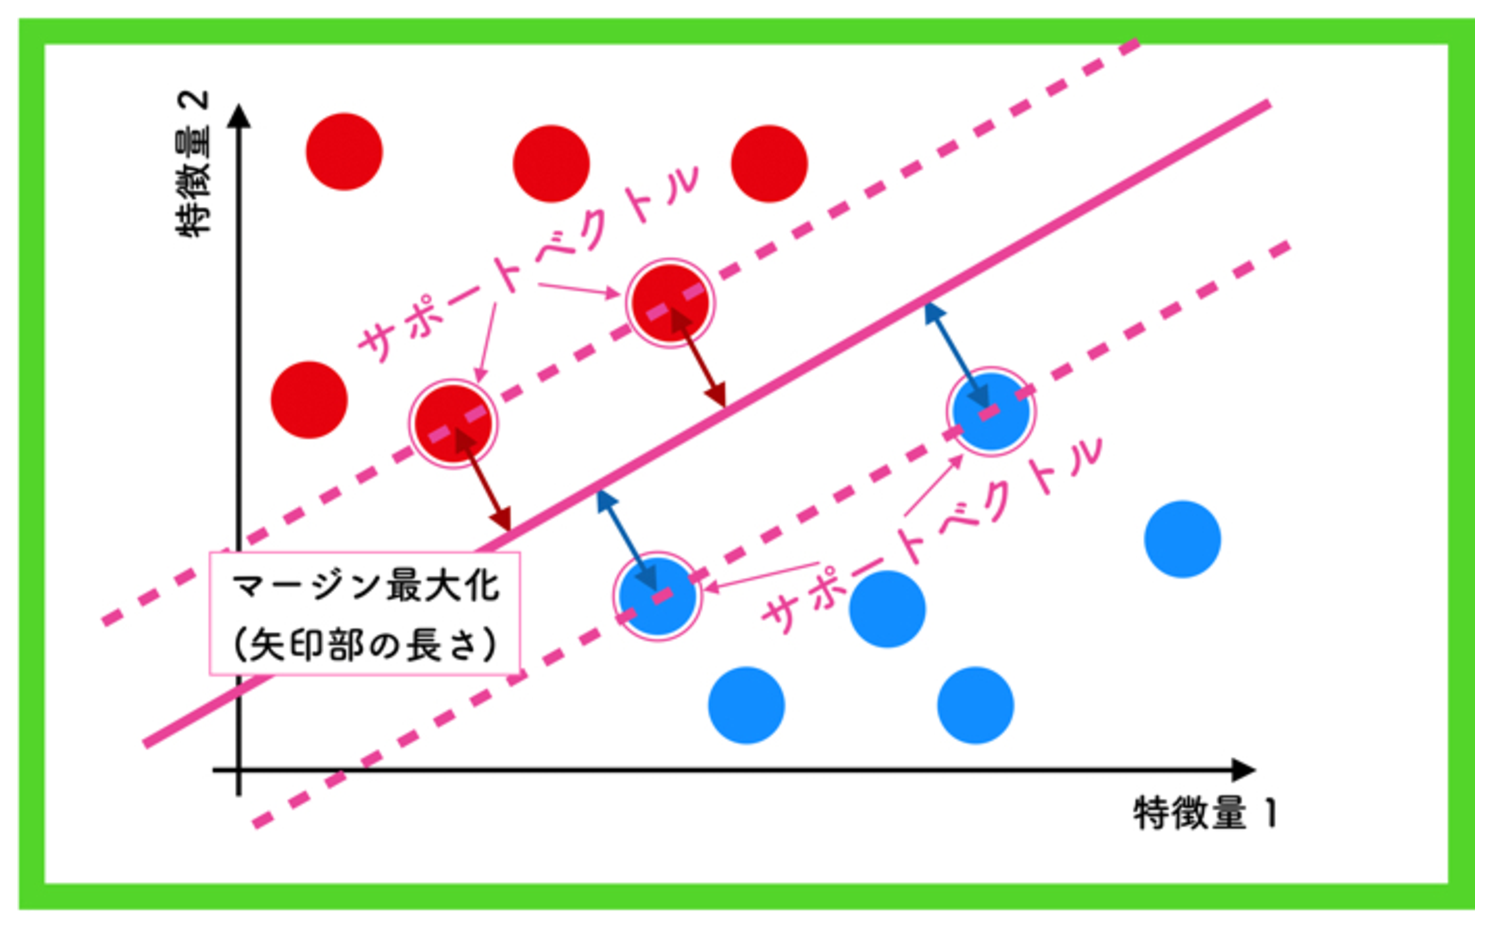
\includegraphics[width=100mm]{./figures/svm/svm.eps}
        \caption{SVMのイメージ図}
    \end{center}
\end{figure}

\subsection*{補足}
SVMはデータの誤分類を許容しない「ハードマージンSVM」と許容する「ソフトマージンSVM」の2種類が存在する.
ハードマージンSVMは,マージン内にデータが存在しないことを前提に考えられており,データがクラス間で重複している場合,識別境界を正確に求められないという問題が生じる可能性がある.
それに対してソフトマージンSVMは,マージン内にデータが存在することやデータの誤分類をある程度許容する代わりに,そのデータにはペナルティを与えるという風に条件を少し緩めることで,多少の重複が存在しても識別できる可能性を上げることを可能としている.\par
では,実際にソフトマージンSVMにおいて,どのようにしてペナルティを与えるのかということに関して簡単に述べる.
まずスラック変数$\zeta$をデータごとに導入する.
$\zeta$はデータが正しく分類されてかつマージン内に存在しない場合は0,正しく分類されているがマージン内に存在する場合は$0<\zeta \leq 1$,誤って分類された場合は$\zeta>1$となる.
そして,マージンの最大化に際して,このスラック変数$\zeta$をペナルティとして与える.
式は以下のようになる.
\begin{equation}
    \zeta_i=|y_i-(\bm{w}^T\bm{x}+b)|
    \label{zeta}
\end{equation}
\begin{equation}
    C\sum_{i=1}^{N}\zeta_i+\frac{1}{2}||\bm{w}||^2 \qquad (C>0)
    \label{margin}
\end{equation}
この式(\ref{margin})を最小化することが目標である.
ここで$C$はペナルティの影響力を制御するパラメータであり,適当に設定する必要がある.
% 式(\ref{zeta})を見て分かる通り,$\zeta$の定義にも$\bm{w}$が含まれている.
誤分類が多くなると式(\ref{margin})の第1項が大きくなるので,最小化しようとするとなるべく誤分類が少なくなるようにパラメータ$\bm{w}$を調整する.
ちなみに,$C \to \infty$とすると,ペナルティの影響力が$\infty$になる,つまり誤分類が全く許容されなくなるので,ハードマージンSVMとなる.\par
ただし,ソフトマージンSVMは与えるペナルティの大きさなどの調整を行う必要があり,少し複雑になることから,今回はハードマージンSVMの実装を行った.

\subsection*{アルゴリズム}
実際に「制約条件$y_i(\bm{w}^T\bm{x}+b_i) \geq 1$のもとで$\frac{1}{2}||\bm{w}||^2$を最小化する」という問題を解いていく.
この問題は多変数関数の最適化問題なので,ラグランジュ乗数$\alpha_i$を導入することで,ラグランジュの未定乗数法に落とし込むことができる.\par
実際にラグランジュ関数は以下のようになる.
\begin{equation}
    L(\bm{w},b,\alpha)=\frac{1}{2}||\bm{w}||^2-\sum_{i=1}^{N}\alpha_i\{t_i(\bm{w}^T\bm{x}_i+b)-1\}
    \label{Lagrange}
\end{equation}
極値条件より,式(\ref{Lagrange})を$\bm{w}$,$b$でそれぞれ偏微分して0とおくと
\begin{equation}
    \left.\frac{\partial L}{\partial \bm{w}}\right|_{\bm{w}=\hat{\bm{w}}}=\hat{\bm{w}}-\sum_{i=1}^{N}\alpha_it_i\bm{x}_i=0
    \label{con1}
\end{equation}
\begin{equation}
    \frac{\partial L}{\partial b}=\sum_{i=1}^{N}\alpha_it_i=0
    \label{con2}
\end{equation}
また,最適性条件より最適解$\hat{\bm{w}}$に対して以下の条件を満たす必要がある.
\begin{equation}
    \nabla L(\hat{\bm{w}},b,\alpha)=\nabla(\frac{1}{2}||\hat{\bm{w}}||^2)-\sum_{i=1}^{N}\alpha_i\nabla\{t_i(\hat{\bm{w}}^T\bm{x}_i+b)-1\}=0
\end{equation}
この式から以下に示す3つの制約条件が得られる.
\begin{equation}
    t_i(\bm{w}^T\bm{x}_i+b)-1 \geq 0
    \label{KKT1}
\end{equation}
\begin{equation}
    \alpha_i \geq 0
    \label{KKT2}
\end{equation}
\begin{equation}
    \alpha_i\{t_i(\bm{w}^T\bm{x}_i+b)-1\}=0
    \label{KKT3}
\end{equation}
式(\ref{KKT1}),(\ref{KKT2}),(\ref{KKT3})はまとめてKKT条件と呼ばれる.\par
式(\ref{con1})より最適解$\hat{\bm{w}}$は
\begin{equation}
    \hat{\bm{w}}=\sum_{i=1}^{N}\alpha_it_i\bm{x}_i
    \label{con1_a}
\end{equation}
式(\ref{con2}),(\ref{con1_a})を式(\ref{Lagrange})に代入すると
\begin{equation}
    L(\hat{\bm{w}},b,\alpha)=\frac{1}{2}||\hat{\bm{w}}||^2-\hat{\bm{w}}^T\sum_{i=1}^{N}\alpha_it_i\bm{x}_i-b\sum_{i=1}^{N}\alpha_it_i+\sum_{i=1}^{N}\alpha_i
\end{equation}
となり,これを$\alpha$の関数と見ると
\begin{eqnarray}
    \tilde{L}(\alpha)&=&\sum_{i=1}^{N}\alpha_i-\frac{1}{2}||\hat{\bm{w}}||^2\\
    &=&\sum_{i=1}^{N}\alpha_i-\frac{1}{2}\sum_{i=1}^{N}\sum_{j=1}^{N}\alpha_i\alpha_jt_it_j\bm{x}_i^T\bm{x}_j
    \label{dual}
\end{eqnarray}
となる.\par
$\bm{w}$はすでに最適化されており,$b$は$\bm{w}$と$\alpha$から一意に定まるので,あとは$\alpha$を最適化すればよい.
主問題は$\frac{1}{2}||\bm{w}||^2$の最小化より,式(\ref{dual})の最大化を行えばよい.
$\alpha$の制約条件としては式(\ref{con2}),(\ref{KKT2})となる.\par
つまり解くべき問題は「制約条件$\sum_{i=1}^{N}\alpha_it_i=0$,$\alpha_i \geq 0$のもとで$\tilde{L}(\alpha)=\sum_{i=1}^{N}\alpha_i-\frac{1}{2}\sum_{i=1}^{N}\sum_{j=1}^{N}\alpha_i\alpha_jt_it_j\bm{x}_i^T\bm{x}_j$を最大化する」ということになる.
このような問題を双対問題と呼ぶ.